\documentclass{article}

%\usepackage{graphicx}

%\usepackage{amsmath}

\usepackage{gvv-book}

\usepackage{gvv}

%\usepackage{float}

\usepackage{enumitem}

%\usepackage{tfrupee}

%\title{CBSE}

%\usepackage{romannum}

%\date{september 2024}

\begin{document}

\begin{enumerate}
        \item In \figref{fig:circleABC}, $PQ$ is a tangent at point $C$ to a circle with center $O$. If $AB$ is a diameter and $\angle CAB = 30^{\degree}$, find $\angle PCA$.
        \begin{figure}[H]
          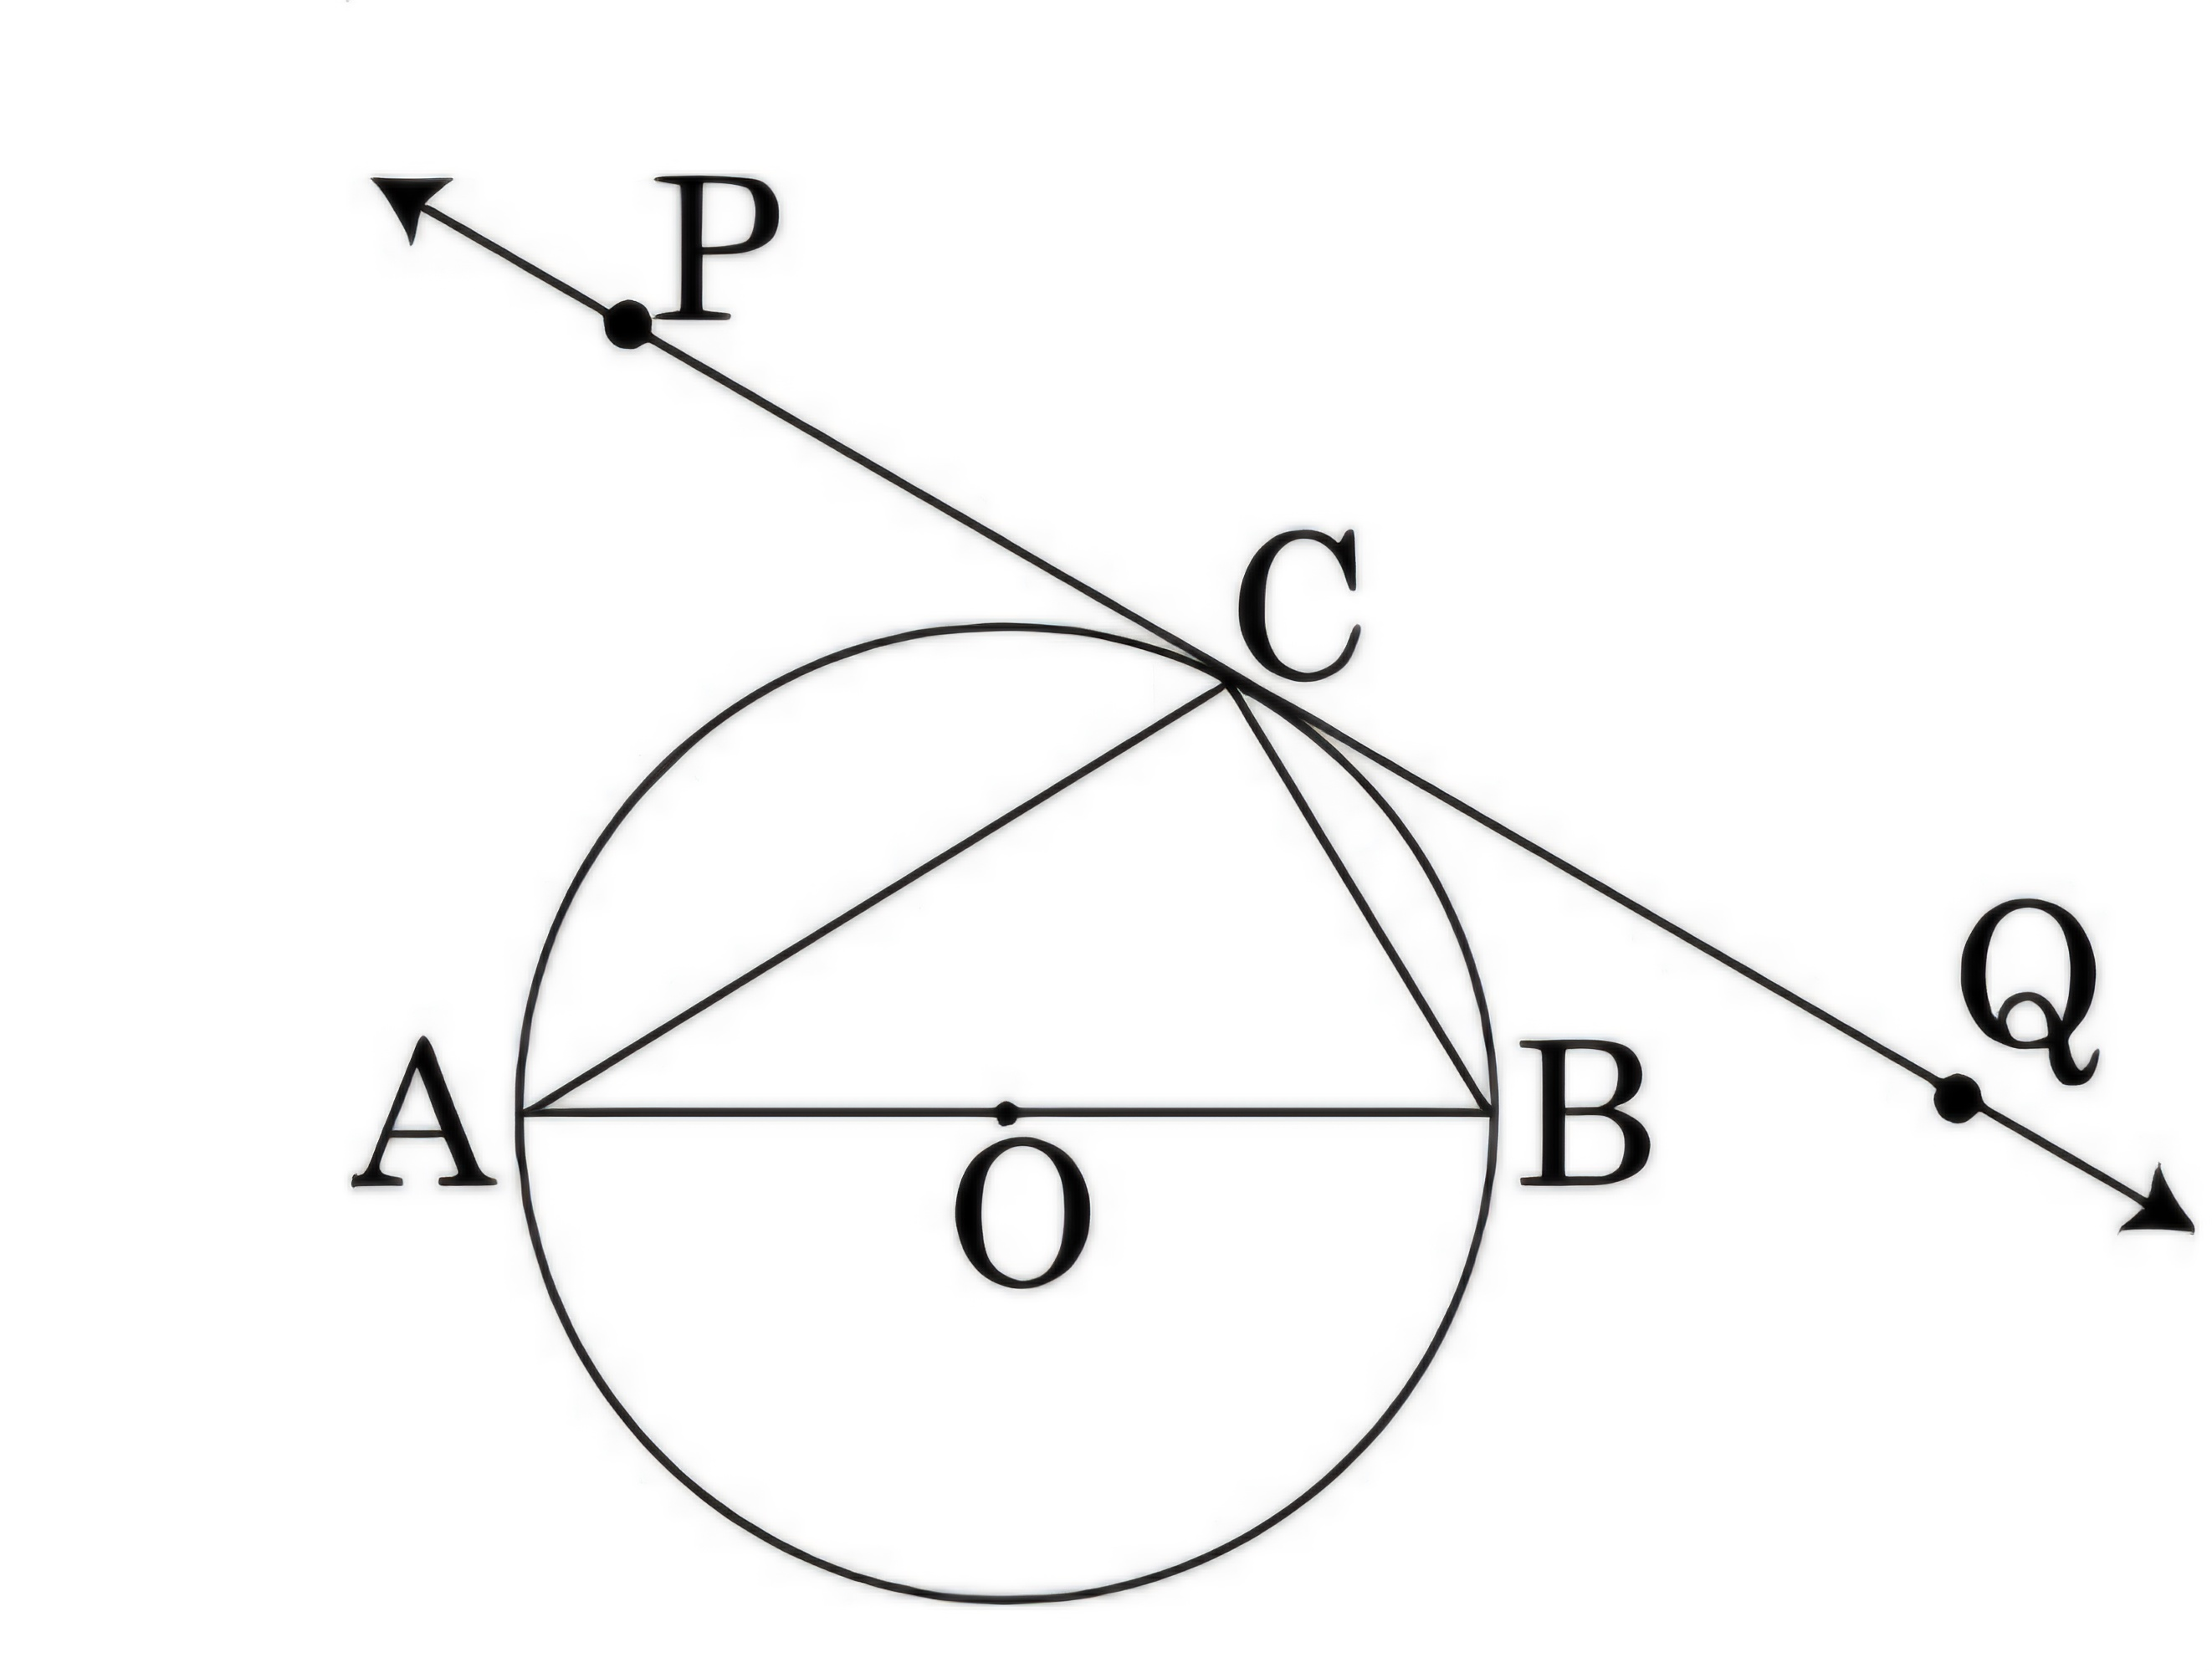
\includegraphics[width=\columnwidth]{./figs/circleABC.jpg}
           \caption{CircleABC}
            \label{fig:circleABC}
         \end{figure}
	 \end{enumerate}
	 \end{document}

	 \item Let $P$ and $Q$ be the points of tr
isection of the line segment joining the
points $A(2, -2)$ and $B(-7,4)$ such that $P$ is nearer to $A$. find the coordinat
es of $P$ and $Q$.

\item In \figref{fig:circle}, $O$ is the centre of a circle such that diameter $AB=13 cm$ and $AC=12 cm$. $BC$ is joined. Find the area of the shaded region. (Take $\pi=3.14$)                               \begin{figure}[H]                          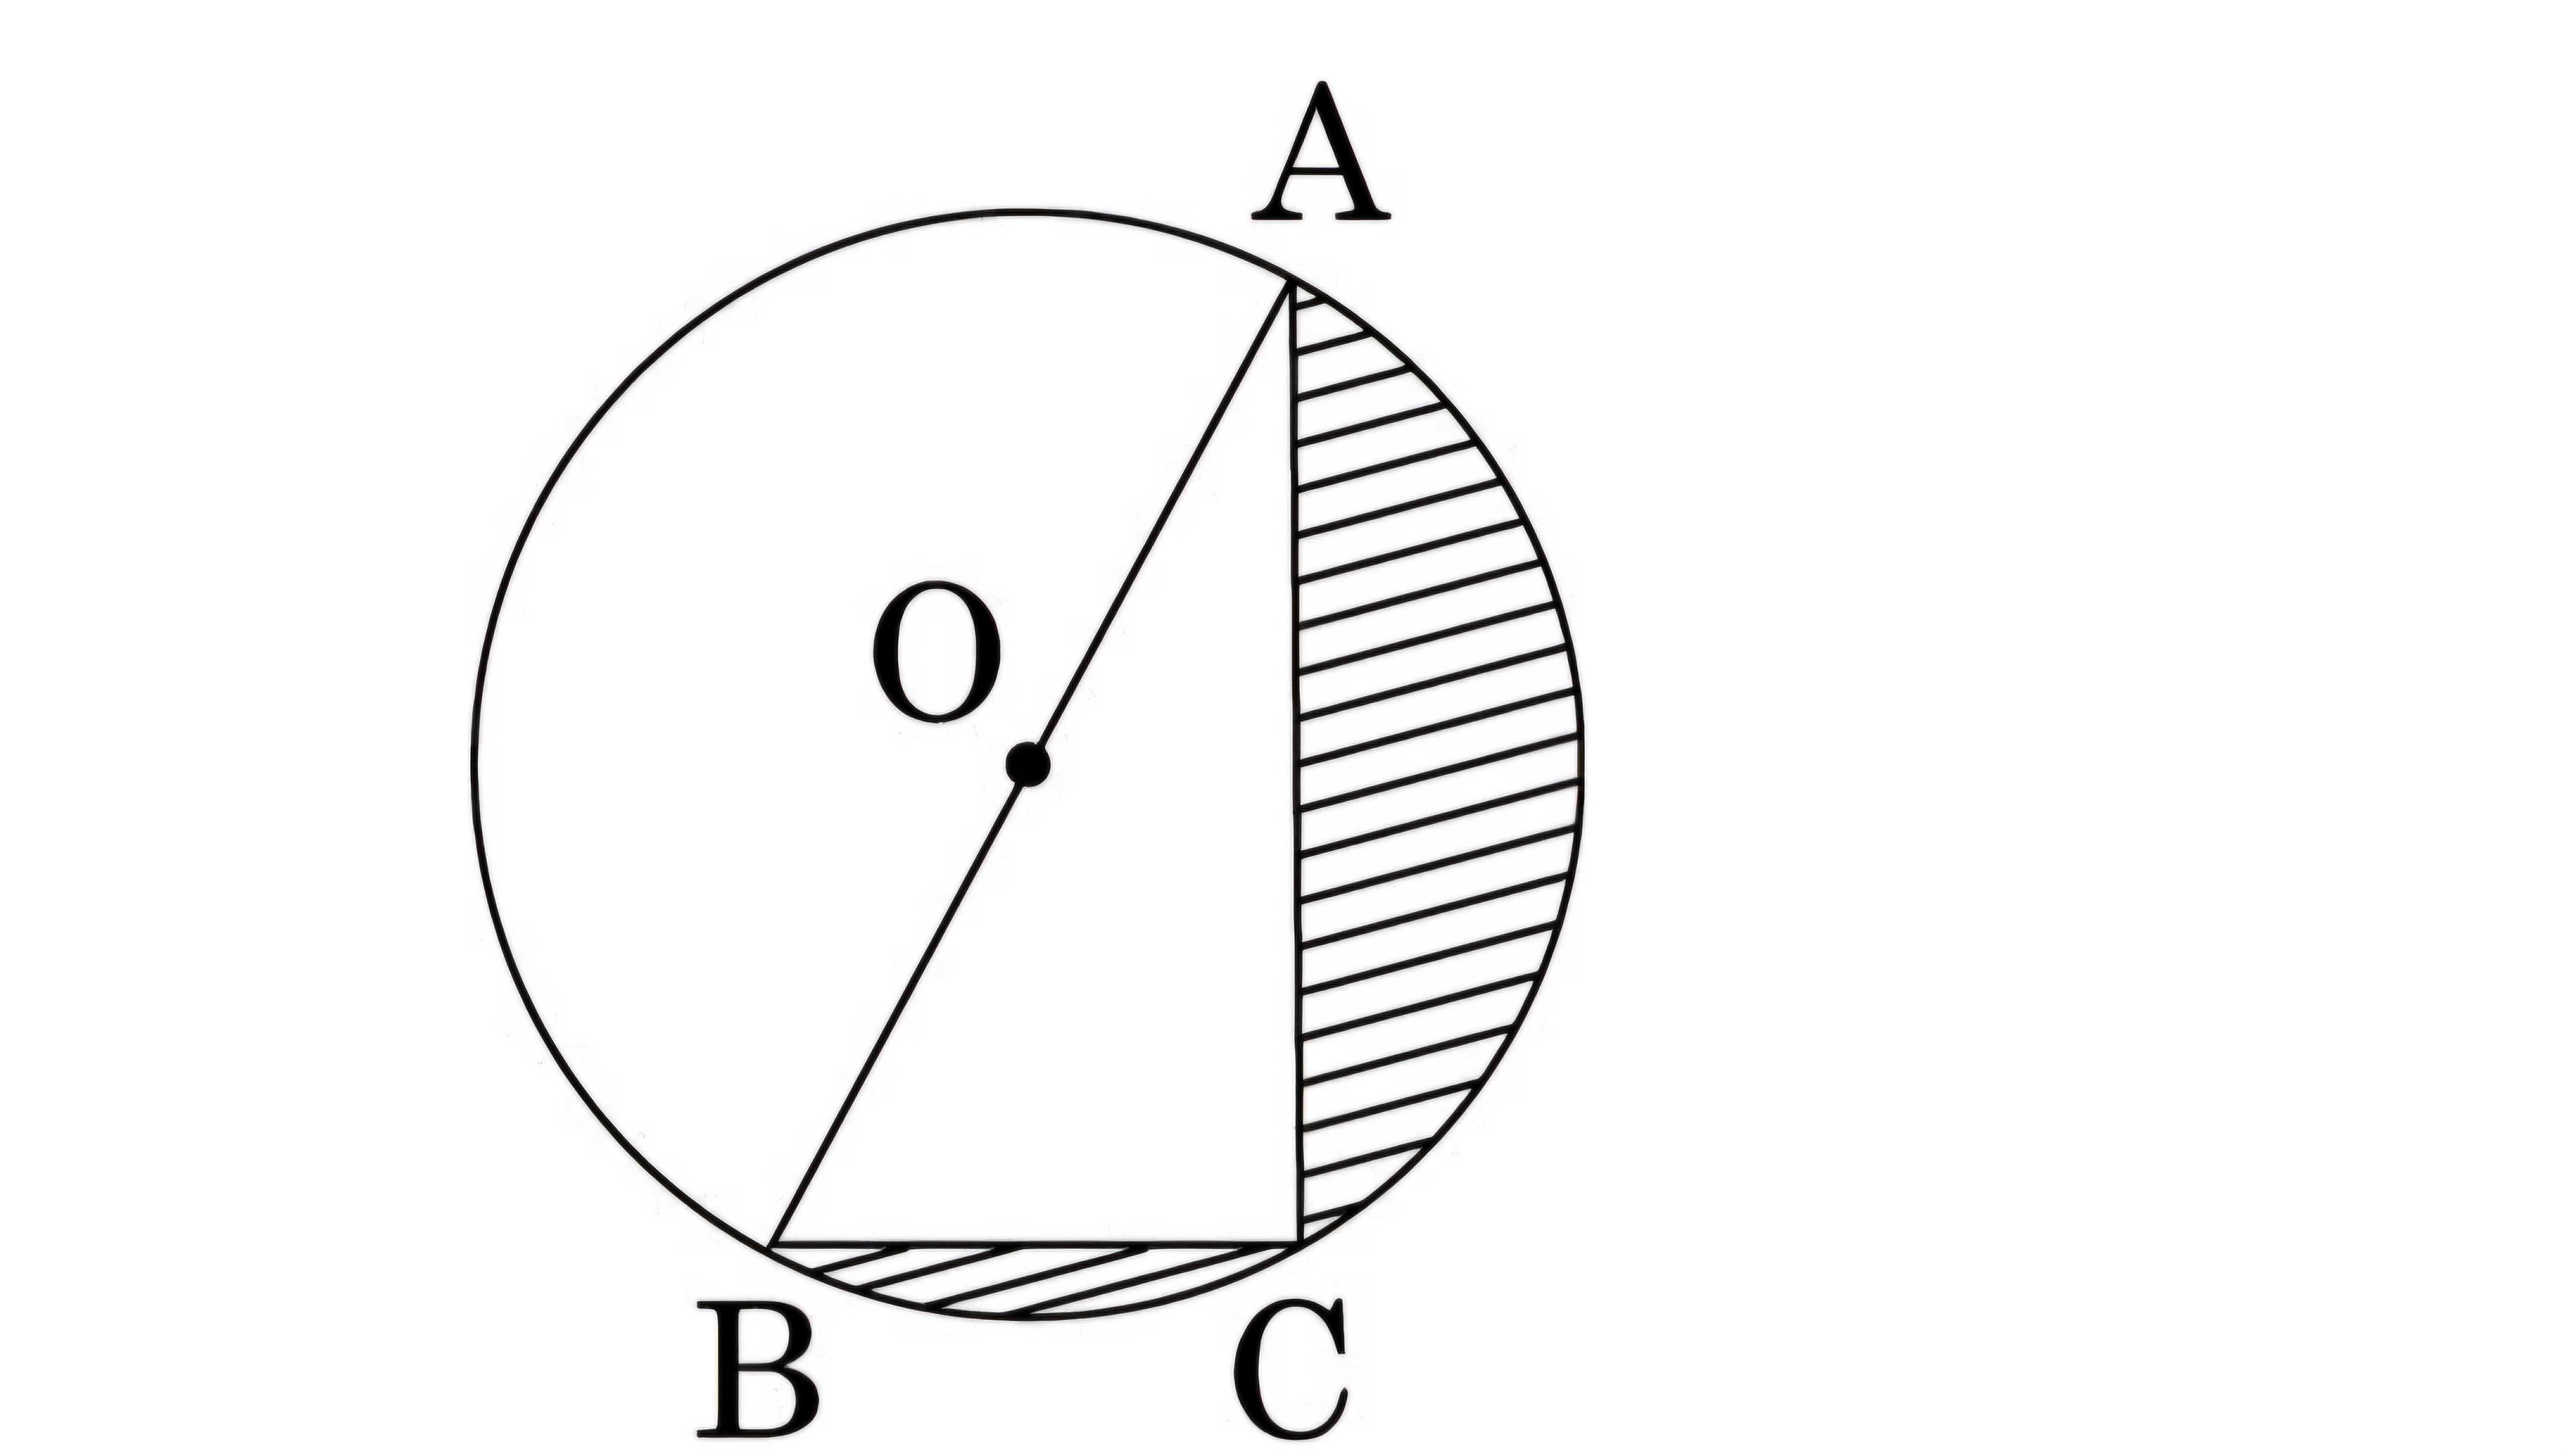
\includegraphics[width=\columnwidth]{./figs/circle.jpg}
    \caption{Circle with centre O}
     \label{fig:circle}                        \end{figure}
     \end{enumerate}
     \end{document}

  \item If the point $P(x, y)$ is equidistant from the points $A(a+b, b-a)$ and $B(a-b, a+b)$. prove that $bx=ay$   

	  \end{enumerate}
	  \end{document}
	  \item Three different coins are tossed together. Find the probability of getting                \begin{enumerate}[label=\roman*]                                     \item exactly two heads,                                                                                                   \item at least two heads


 \item at least two tails.                             \end{enumerate}
	 \end{enumerate}
	 \end{document}
	 \item prove that the lengths of the tangents drawn from an external point to a circle are equal.
		 \end{enumerate}
		 end{document}
\item Drawn a circle of radius $4 cm$. Drawn two tangents to the circle inclined at an angle of $60^{\degree}$ to each other.
	\end{enumerate}
	\end{document}
